\documentclass[12p]{article}
\usepackage[margin=1in, headheight=110pt]{geometry}
\usepackage{amssymb, amsmath, amsfonts, amsthm}
\usepackage{mathpazo}
\usepackage{setspace}
% \usepackage{probsoln}
\usepackage{fancyhdr}
\usepackage{hyperref}
\usepackage{float}
\usepackage{tikz}
\usepackage{enumitem}
\usepackage{graphicx}
\usepackage{listings}
\usepackage{caption}
\usepackage{bookmark}

\def\ojoin{\setbox0=\hbox{$\bowtie$}%
  \rule[-.02ex]{.25em}{.4pt}\llap{\rule[\ht0]{.25em}{.4pt}}}
\def\leftouterjoin{\mathbin{\ojoin\mkern-5.8mu\bowtie}}
\def\rightouterjoin{\mathbin{\bowtie\mkern-5.8mu\ojoin}}
\def\fullouterjoin{\mathbin{\ojoin\mkern-5.8mu\bowtie\mkern-5.8mu\o}}

\pagestyle{fancy}
\lhead{Evan Quan, Irene Chan, Patrick Gharib}
\rhead{SENG 300 - Group Project Iteration 1 - Winter 2018}
\title{\vspace{-6ex}Groupd Project Iteration 1}
\date{\vspace{-12ex}}


\newcommand{\code}[1]{\texttt{#1}}

\setlength{\parindent}{0pt}
\begin{document}
% \maketitle
\thispagestyle{fancy}

\begin{titlepage}
  \begin{center}
    \vspace{1cm}
    \Large{\textbf{University of Calgary}}\\
    \Large{\textbf{SENG 300  - Introduction to Software Engineering}}
    \vfill
    \line(1,0){400}\\[1mm]
    \huge{Group Project Iteration 1}\\
    \large{Finding Declarations and References}\\
    \line(1,0){400}\\
    \Large March 14, 2018\\
    \vfill
    \large{Evan Quan, Irene Chan, Patrick Gharib}\\
  \end{center}
\end{titlepage}

\tableofcontents
\thispagestyle{empty}
\clearpage

\onehalfspacing

\setcounter{page}{1}

\newpage
\section{Structural Diagram}
% \begin{figure}[H]
%   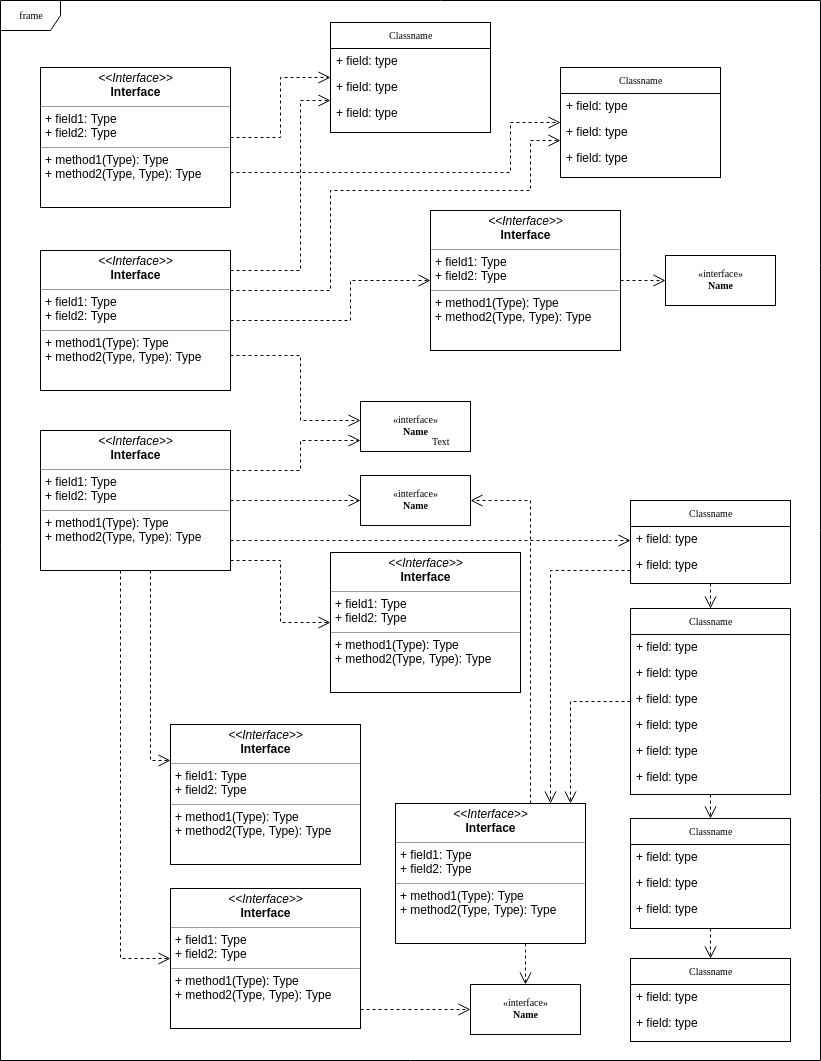
\includegraphics[width=1.0\textwidth]{Structure.png}
%   \caption{}
%   \label{fig:structural}
% \end{figure}


\newpage

\section{Sequence Diagram}
% \begin{figure}[H]
%   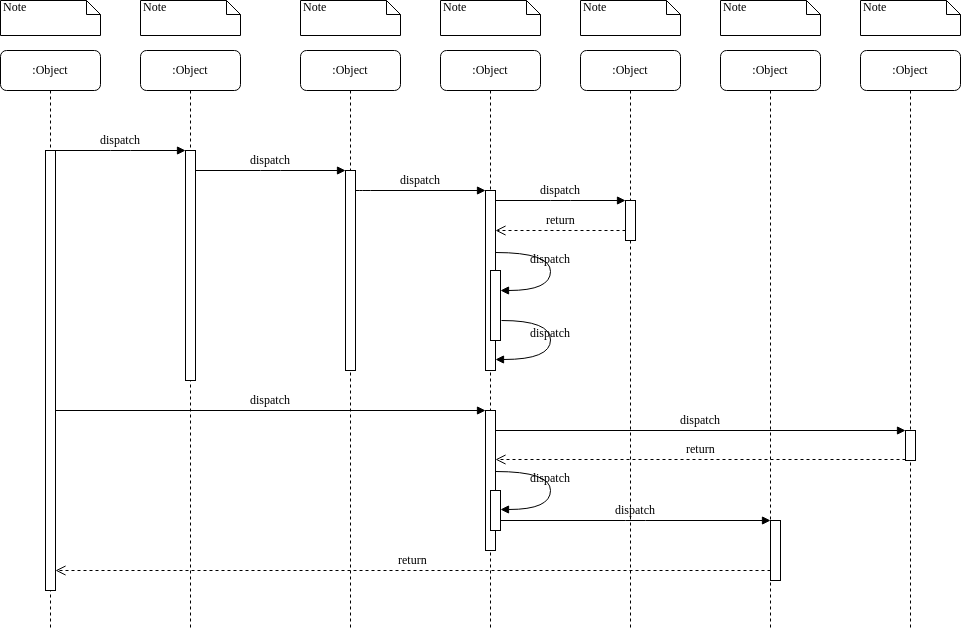
\includegraphics[width=1.0\textwidth]{Sequence.png}
%   \caption{}
%   \label{fig:sequence}
% \end{figure}


\newpage

\section{State Diagram}
% \begin{figure}[H]
%   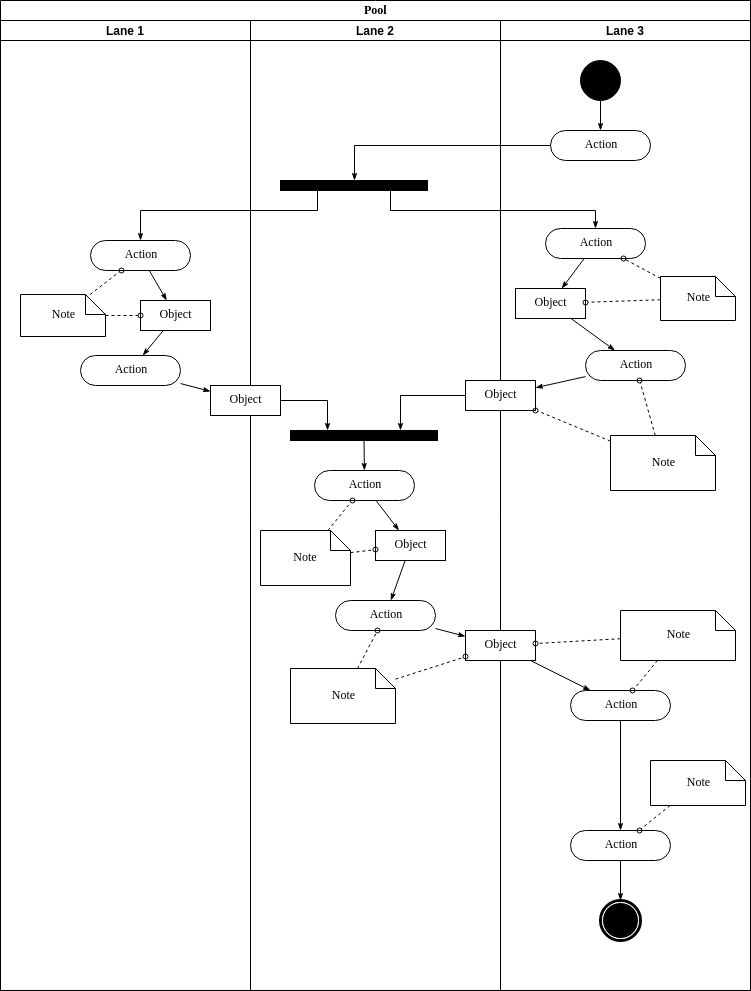
\includegraphics[width=1.0\textwidth]{State.png}
%   \caption{}
%   \label{fig:state}
% \end{figure}
\end{document}
